\subsection{Introduction}
As already stated in the previous chapters, it is well-known that in general the electrophysiological
signal (acquired from a single electrode) is characterized by 2 distinct patterns:
\begin{itemize}
    \item \textbf{Spike:} a single over-threshold signal representing the activity of one or
    more neurons (typically a so-called unit or channel).
    \item \textbf{Burst:} a sequence of highly packed spikes often occurring simultaneously on
    several channels and giving rise to a phenomenon known as network burst.
\end{itemize}
\begin{figure}[H]
    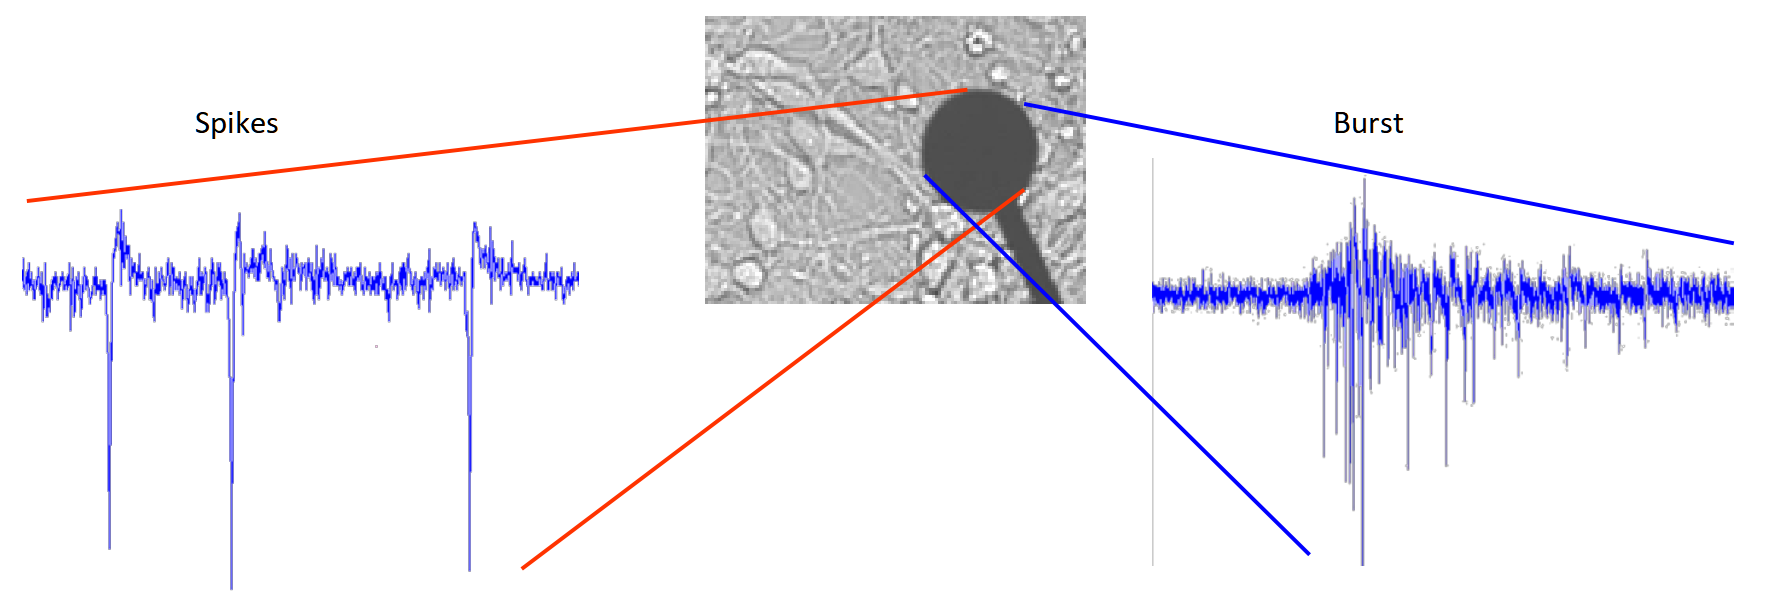
\includegraphics[scale=0.4]{4_1}
    \centering
\end{figure}


\subsection{Data visualization tools}
The first preliminary steps of Spike Analysis consist in taking a look at the raw data, then
deriving the spike train for each channel and visualize it. Therefore, it might be useful to define
a set of proper plots and metrics for data visualization.
\subsubsection{Raw data multi-channel plot}
The following plot shows the activity - i.e. voltage - recorded by 8 distinct electrons as a
function of time.
\begin{figure}[H]
    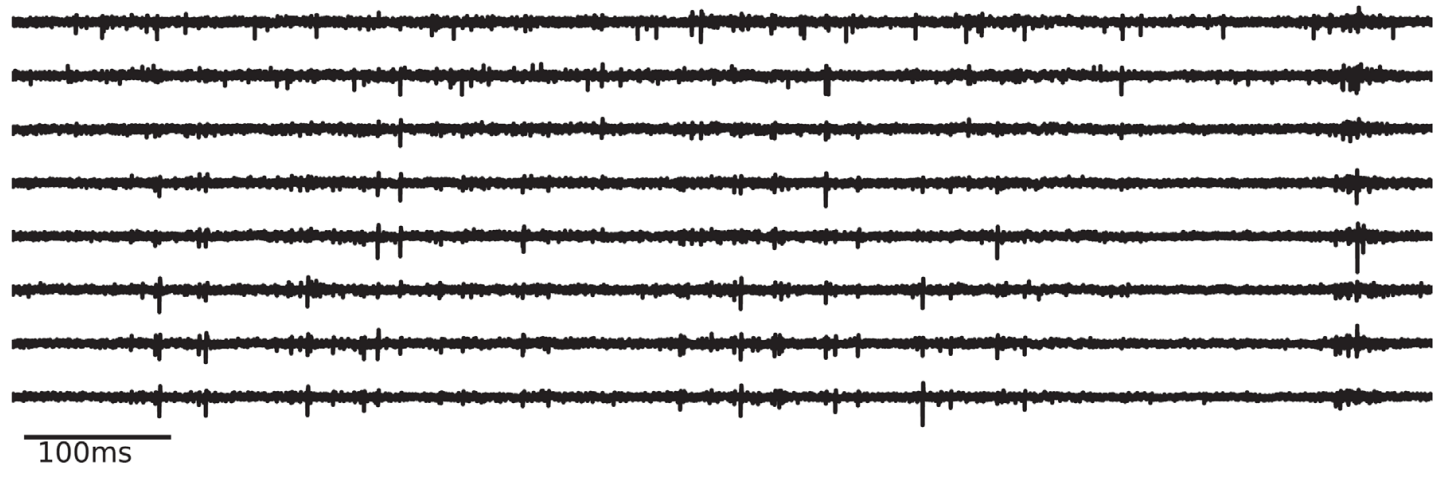
\includegraphics[scale=0.4]{4_2}
    \centering
\end{figure}
\subsubsection{Raster Plot}
The Raster Plot (also known as Spike Raster) is done after Spike Sorting and it allows to visualize
at the same time the spike trains coming from multple recording electrodes on the same time axis.
It is common to observe consistent activation patterns across channels, as neurons influence each
other.
\begin{figure}[H]
    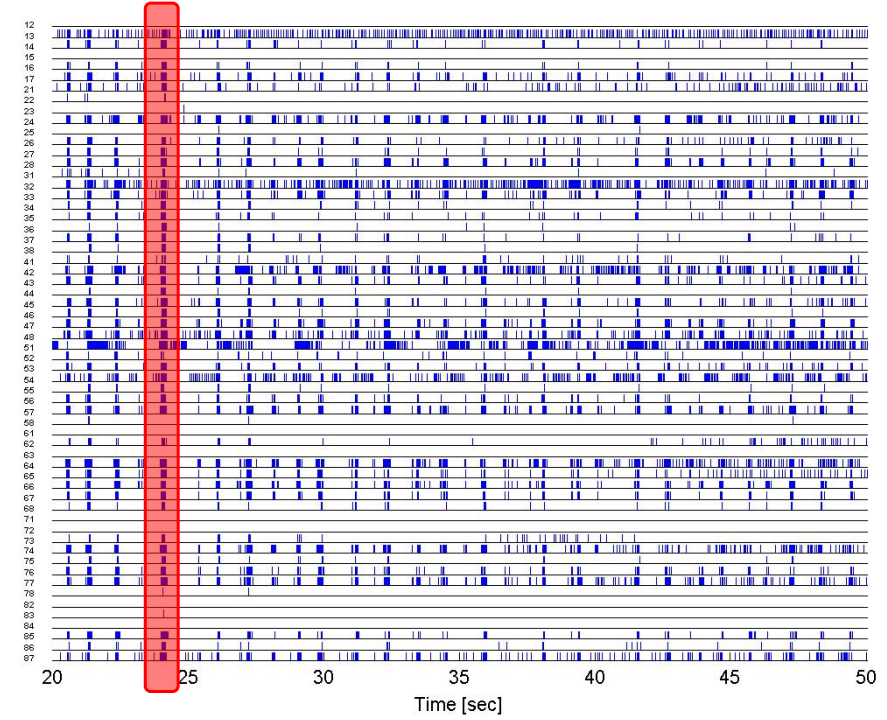
\includegraphics[scale=0.75]{4_3}
    \centering
\end{figure}
\subsubsection{Task-Related Raster Plot}
The Task-Related (or Stimulus-Related) Raster Plot is similar to the ordinary Raster Plot, even if it
has a quite different meaning: the multiple lines do not represent channels, but portions of the
recording coming from just one channel. The signal portions are divided according to the execution of
a task or the receiving of a stimulus.
\begin{figure}[H]
    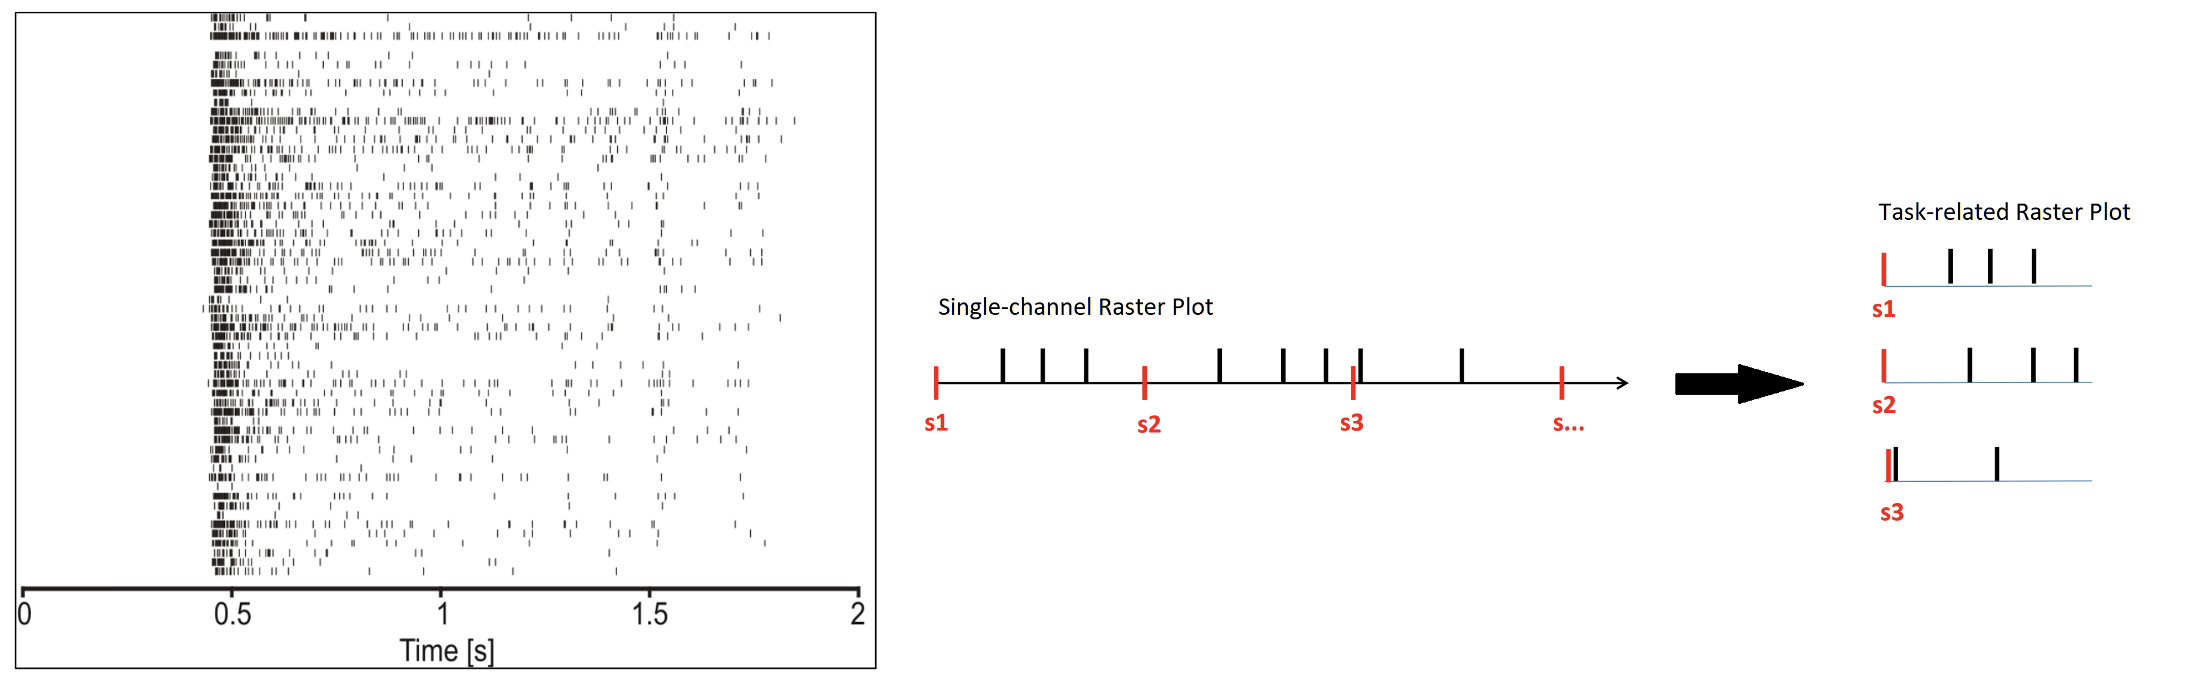
\includegraphics[scale=0.4]{4_4}
    \centering
\end{figure}
\subsubsection{High-Density Data Raster Plot}
This is once again a type of Raster Plot. Data comes from several channels and they cover a relatively
large span of time. As a consequence, it is almost impossible to distinguish single spikes by eye,
thus this high-density plot is usually inspected by looking at the shaded regions, as they exhibit a
higher concentration of fired spikes, implying a greater activity.
\begin{figure}[H]
    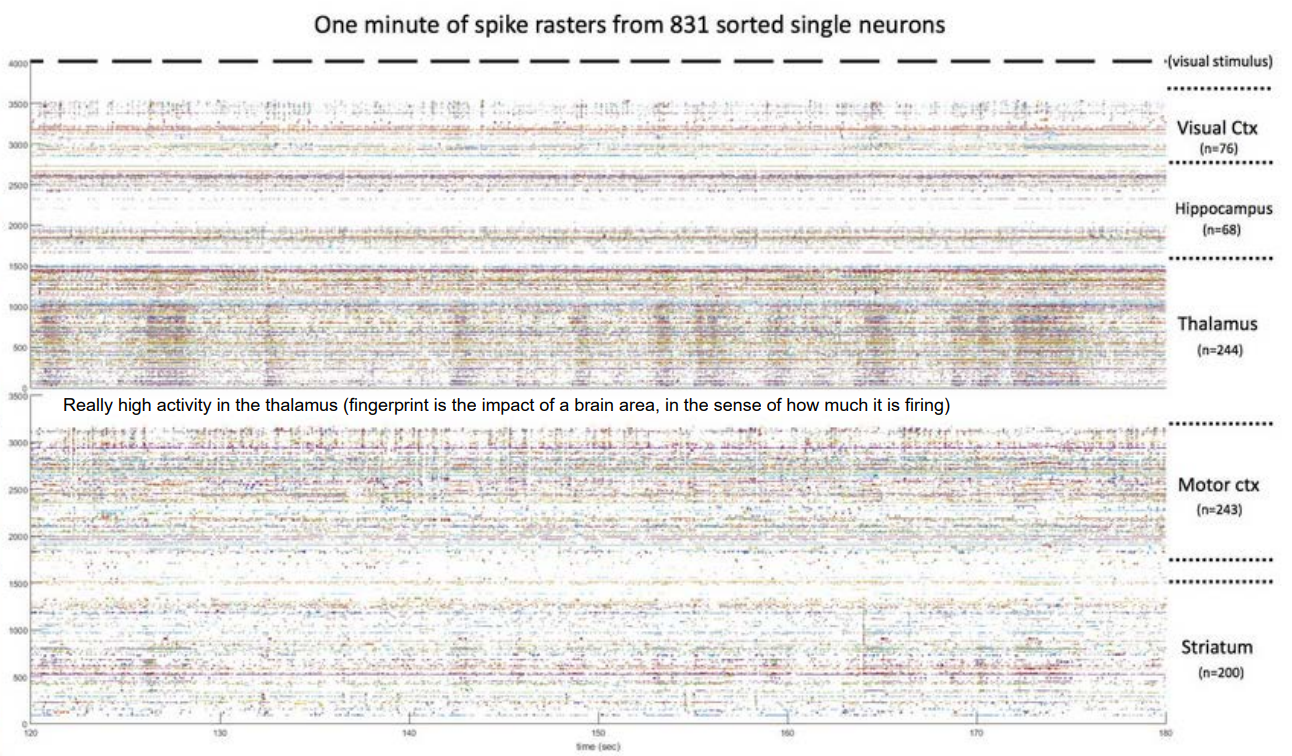
\includegraphics[scale=0.6]{4_5}
    \centering
\end{figure}
\subsubsection{Spike Count and Firing Rate metrics}
\paragraph{Spike Count}
This metric is obtained by dividing the time axis into equal bins \(\Delta{t}=[t_a,t_b]\) and just
counting the number of spikes \(N_{ab}\) occurring in each bin.
Then, an histogram showing the Spike Count can be plotted.
\paragraph{Instantaneous Firing Rate}
By simply taking the Spike Count and dividing it by the bin size, the Instantaneous Firing Rate (IFR)
can be derived. 
\begin{align*}
    IFR=r(t)=\frac{N_{ab}(t)}{\Delta{t}}
\end{align*}
The IFR is measured in spikes per second.
\paragraph{Spike Density Function}
The Spike Density Function (SDF) is obtained by associating a proper distribution (typically Gaussian)
to each single spike, then the SDF is derived by summing up the various individual distributions.
\begin{figure}[H]
    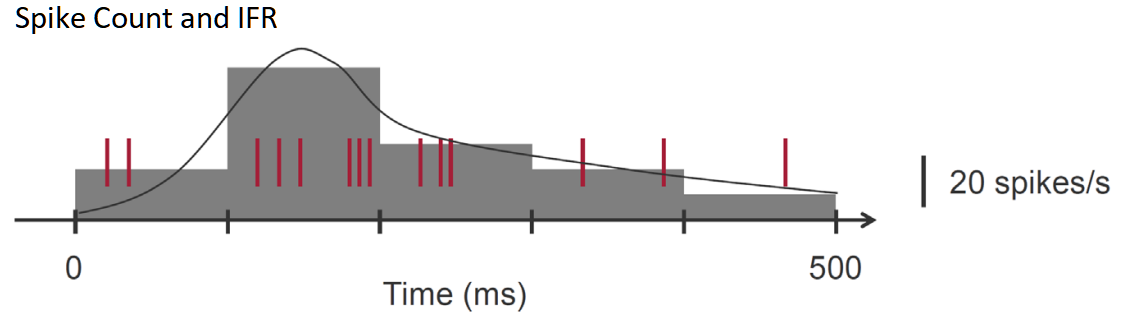
\includegraphics[scale=0.6]{4_6}
    \centering
\end{figure}
\paragraph{Array-Wide Firing Rate}
The Array-Wide Firing Rate (AWFR), often called Average Firing Rate (AFR), it is a sort of
IFR by taking into account the whole network - i.e. all the recorded channles, not just a single one.
This metric is often employed in neuropharmacology, in order to assess the time of response of a drug.\\
By setting the number of channels - i.e. the number of electrodes - to \(M\), the AFR is defined as:
\begin{align*}
    AWFR=awfr(t)=mean(IFR)=\frac{1}{M}\sum_{j=1}^{M}r_{j}(t)
\end{align*}
\paragraph{Mean Firing Rate}
The Mean Firing Rate (MFR) represents a single numerical metric of the activity of neurons for the
entire network (\(M\) channels). It is expressed as
\begin{align*}
    MFR=\frac{1}{T}\sum_{j=1}^{M}N_j
\end{align*}
where \(T\) is the considered time window (somehow corresponding to the previously seen \(\Delta{t}\)),
while \(N_j\) is the number of spikes recorded in the \(T\) interval for the \(j\)-th electrode.\\
Notice once again that both IFR and AWFR are functions of time, continuous in the time-domain, while
MFR is a single value giving information on the average degree of activation of the whole neural
network in a determined time interval.\\
The following plot illustrates the Mean Firing Rate, indicating the average neural activity, at
different concentrations of a brain inhibitor drug.
\begin{figure}[H]
    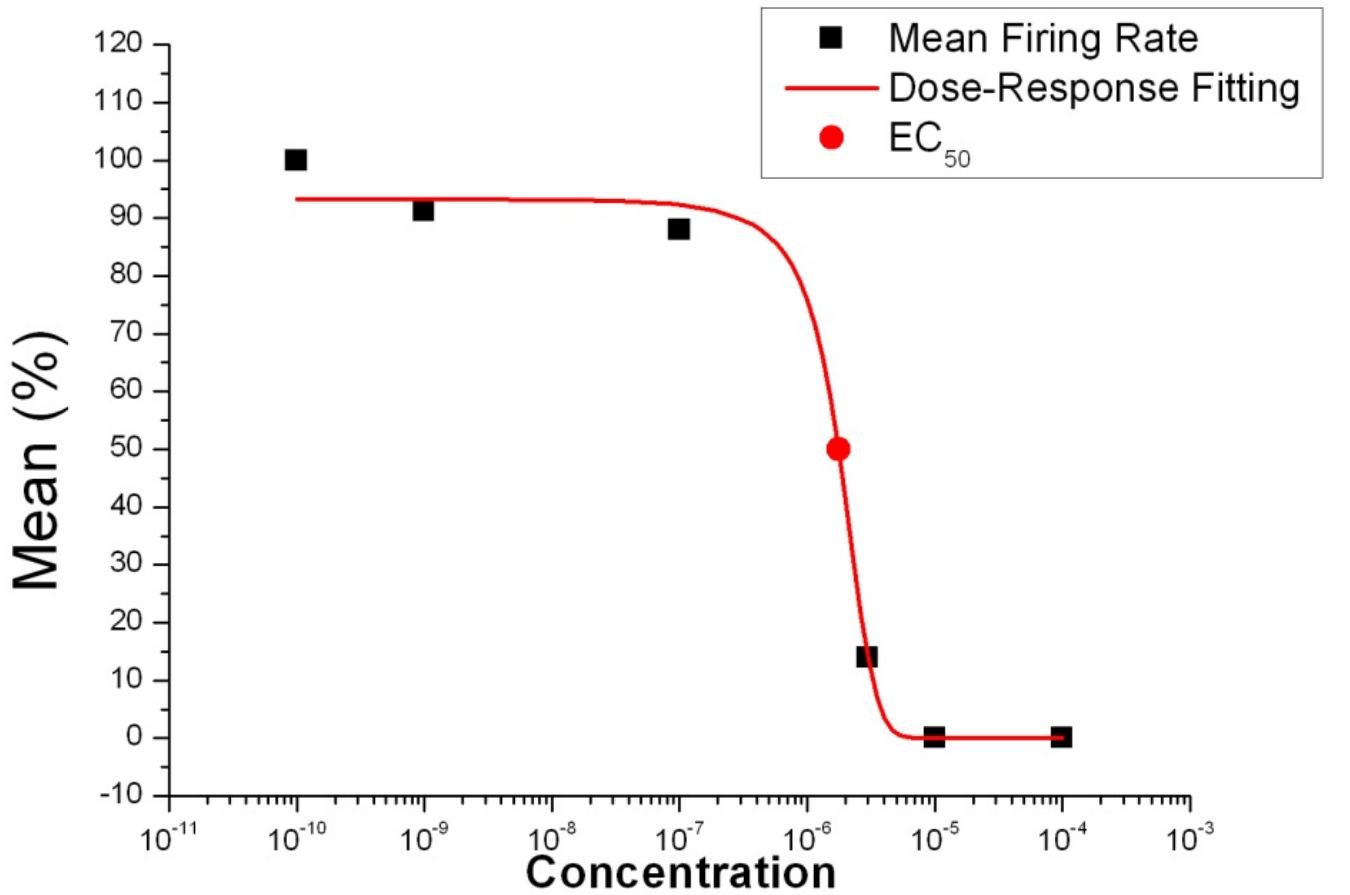
\includegraphics[scale=0.35]{4_7}
    \centering
\end{figure}
\subsubsection{Inter Spike Interval}
\paragraph{Inter Spike Interval}
The Inter Spike Interval (ISI) is the interval between two consecutive spikes. It is used to compute
the Inter Spike Interval Histogram (ISIH), an index of the probability that a spike is fired
a certain time \(\tau\) after a reference spike.
Given \(N\) spikes, the ISIH metric is computed as shown below:
\begin{align*}
    ISIH(\tau)=\frac{1}{N-1}\sum_{s=1}^{N-1}\delta{(t_{s+1}-t_{s}-\tau)}
\end{align*}
An histogram as the following one is often employed to visualize the metric.
\begin{figure}[H]
    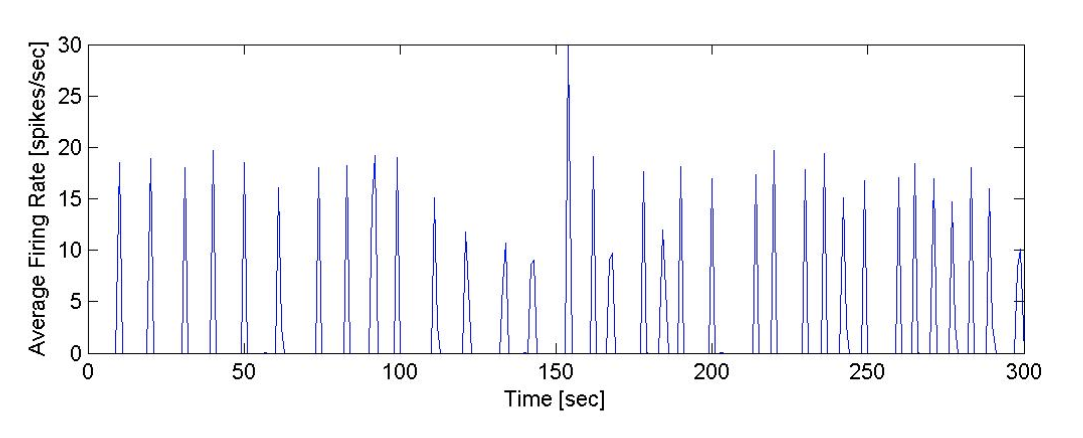
\includegraphics[scale=0.5]{4_8}
    \centering
\end{figure}
Notice that it is common to have a higher probability close to the reference spike, while it tends to
decrease as the Inter Spike Interval grows. If the spike train is made of packed spikes alternating
to empty intervals, then the histogram will display 2 distinct peaks: one for the high frequency
component and one for the low frequency component.
\paragraph{Joint Inter Spike Interval}
The Joint Inter Spike Interval (JISI) is derived from the ISI and it is useful to evaluate the
relationship between pre-ISI and post-ISI intervals, for any spike of the train.
The probability JISIH for \(N\) spikes is computed as:
\begin{align*}
    JISIH(\tau_{post},\tau_{pre})=\frac{1}{N-2}\sum_{s=2}^{N-1}\delta{(t_{s+1}-t_{s}-\tau_{post})}\ast \delta{(t_s-t_{s-1}-\tau_{pre})}
\end{align*}
In this case the plot becomes tridimensional, however it can be displayed in 2D by using
colormaps.
\begin{figure}[H]
    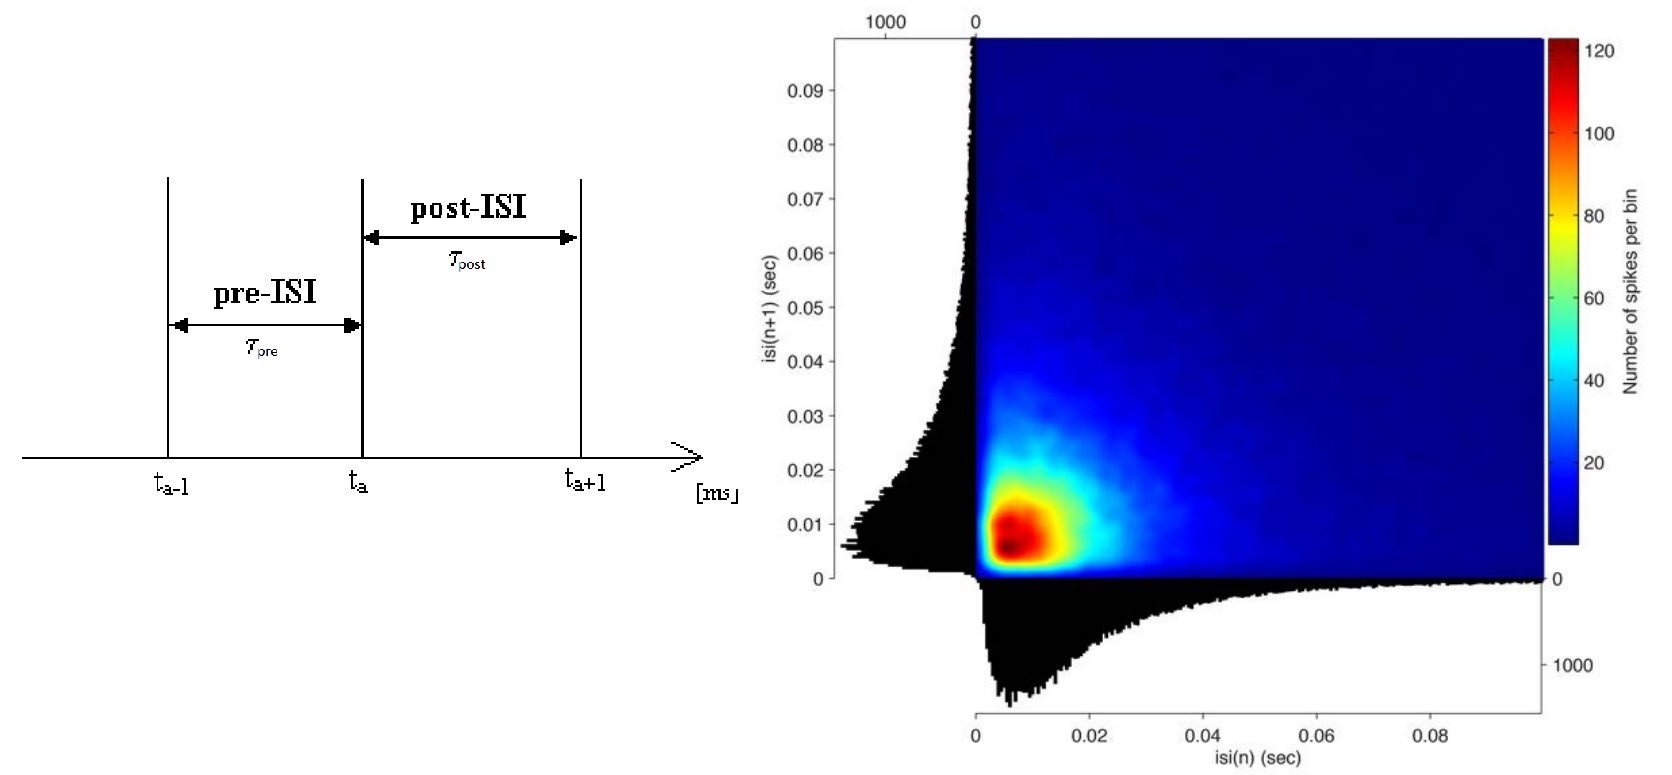
\includegraphics[scale=0.45]{4_9}
    \centering
\end{figure}
\paragraph{Cross Inter Spike Interval}
The Cross Inter Spike Interval (CISI) works in a fashion similar to JISI, but it analyzes the
dependance between spikes of two different trains. The probability CISIH is given by:
\begin{align*}
    CISIH(\tau_{post},\tau_{cross})=\frac{1}{N-2}\sum_{a=1}^{N_a-1}\delta{(t_{a+1}-t_{a}-\tau_{post})}\ast \delta{(t_a-t_b-\tau_{cross})}
\end{align*}
\begin{figure}[H]
    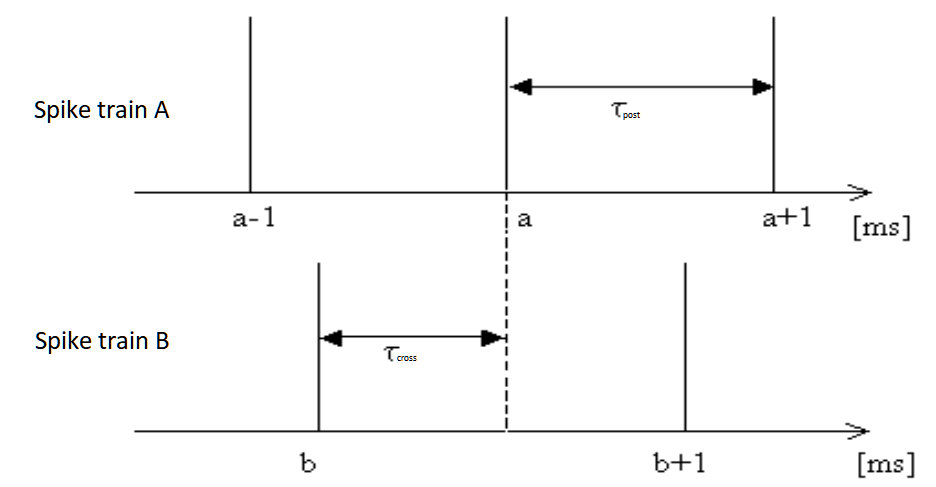
\includegraphics[scale=0.5]{4_10}
    \centering
\end{figure}